\section{Candidate Preselection}
\label{sec:Preselection}

\subsection{Candidate building and preselection on derivation level}
\label{ssec:CandidateBuildingByDerivation}

For the Run~2 \Bmumu\ analysis the \Bds\ and \Jpsi\ candidates are build
simultaneously by the derivation format \texttt{BPHY8} (for data and continuum
background) in the three relevant decay modes:
\begin{itemize}
\item \Bmumu\ signal channel\\
  A \Bds candidate is build from two oppositely-charged muons.  
  Before vertexing the muon momenta are corrected by the 
  \texttt{MuonCalibrationAndSmearingTool} as
  recommended by the muon combined performance group, applying the 
  appropriate configurations\footnote{
    %% w.w., 2018-04-13:
    %% Please note that these are already the updated settings for
    %% the upcoming re-processing of all our DAODs.
    For data15: 
    \texttt{McstYear = ``Data15''}, 
    \texttt{McstRelease = ``Recs2017\_08\_02''},
    \texttt{McstStatComb = False},
    \texttt{McstSagittaCorr = True},
    \texttt{McstSagittaRelease = ``sagittaBiasDataAll\_25\_07\_17''},
    \texttt{McstDoSagittaMCDistortion = False};\newline
    for data16:
    \texttt{McstYear = ``Data16''}, 
    \texttt{McstRelease = ``Recs2017\_08\_02''},
    \texttt{McstStatComb = False},
    \texttt{McstSagittaCorr = True},
    \texttt{McstSagittaRelease = ``sagittaBiasDataAll\_25\_07\_17''},
    \texttt{McstDoSagittaMCDistortion = False};\newline
    for MC the data16 settings are applied.
  }
  for data15 and data16.
  Using the \texttt{JpsiFinder} tool, the \Bds\ candidates are 
  constructed by a fit of the two muon's inner detector tracks to a
  common vertex requiring $\chi^2_{\Bds}/NDF < 15$ and $3500~\mathrm{MeV} 
  < m_{\Bds} < 7000~\mathrm{MeV}$.  In addition, the so called
  muon-based mass $m^{\mathrm{MUCALC}}_{\Bds}$ and the corresponding 
  uncertainty are calculated as the invariant
  mass from the four-momentum sum using the combined muon
  information of the two muons comprising the candidate.  The
  PDG-mass for muons is applied in this calculation.
  On data, the candidates two mass values are 
  \yel[The footnote text already explains the new blinding method
  with the encrypted mass values.]{blinded}\footnote{
    The mass values are encrypted using a simple RSA algorithm with 
    asymmetric keys, multiplied by $-1$, so that they 
    appear on the negative side of the mass spectrum, 
    and stored in the same float variable.
  }
  if both, $m_{\Bds}$ and $m^{\mathrm{MUCALC}}_{\Bds}$ fall into the blinded
  region around the nominal $\Bs$, i.e. into the interval from
  5166~MeV to 5526~MeV.
\item \BpmKpmJpsi\ reference channel with \JpsiMuMu\\
  First \Jpsi\ candidates are reconstructed using the
  \texttt{JpsiFinder} similarily as for the \Bmumu\ signal channel
  with an adjusted mass range of
  $2000~\mathrm{MeV} < m_{\Jpsi} < 7000~\mathrm{MeV}$.
  Then the \texttt{JpsiPlus1TrackFinder} tool is used to combine the \Jpsi\ 
  candidates with an additional track\footnote{
    We apply the BLS group's standard inner detector track preselection
    for vertexing as defined in \texttt{configureVertexing.py}, among
    them 
    \texttt{pTMin = 400.0}~MeV,
    and the minimal track hit requirements
    \texttt{nHitBLayer = 0}, 
    \texttt{nHitPix = 1},
    \texttt{nHitBLayerPlusPix = 1},
    \texttt{nHitSct = 2},
    \texttt{nHitSi = 3},
    \texttt{NHitTrt = 0} 
    as well as
    \texttt{TrtMaxEtaAcceptance = 1.9}.
  }
  which is required to have  
  $\pt^{Jpsi} > 1$~GeV and $|\eta < 2.5|$.  A mass constraint of the \Jpsi\
  candidate's mass to the \Jpsi\ PDG mass is applied. 
  The \Bpm\ candidates are 
  accepted if $\pt^{\Bpm} > 1$~GeV, $\chi^2_{\Bpm}/NDF < 15$ and
  $3500~\mathrm{MeV} < m_{\Bpm} < 7000~\mathrm{MeV}$.
  Again, muon-based mass values $m^{MUCALC}_{\Bpm}$ and corresponding 
  uncertainties are calculated
  from the four-momenta of the two muons and the additional kaon
  track, assuming PDG values for the masses of the muons and the kaon
  as appropriate.  No mass-value blinding is applied to the reference
  channel candidates.
\item \BsJpsiPhi\ control channel with \JpsiMuMu\\
  To reconstruct \BsJpsiPhi\ candidates, the \Jpsi\ candidates
  reconstructed as described for the  \BpmKpmJpsi\ channel above are
  combined with two oppositely-charged inner detector tracks
  fulfilling the same requirements as the kaon track in the
  \BpmKpmJpsi\ reconstruction by the \texttt{JpsiPlus2TracksFinder}
  tool. Again, a mass constraint of the \Jpsi\ candidate's mass to the
  \Jpsi\ PDG mass is applied.
  Muon-based mass values $m^{MUCALC}_{\Bs}$ and corresponding 
  uncertainties are calculated
  from the four-momenta of the two muons and the two additional kaon
  tracks, assuming PDG values for the masses of the muons and the kaons
  as appropriate.  No mass-value blinding is applied to the control
  channel candidates.
\end{itemize}

For MC signal channels only the relevant decay modes are run.  For
the \Bhh\ MC the requirement that the inner detector tracks must be
identified as muons is dropped. Instead two oppositely-charged tracks
with $\pt > 3.5$~GeV and $|\eta| < 2.5$ are required.
For the \BpPipJpsi\ Monte Carlo sample, two instances of the
\BpmKpmJpsi\ mode are run in parallel.  The first one is assuming the
PDG pion mass for the additional track, while the second one assumes
the (wrongly-assigned) PDG kaon mass.  The second version is needed as
-- due to the lack of pion-kaon separation in ATLAS -- 
our \BpmKpmJpsi\ reference sample on data will contain a contribution
of \BpPipJpsi\ events located to the right of the \Bpm\ peak 
due to the wrongly-assigned mass values for the pion track.

At derivation level each $B$ and $\Jpsi$ candidate is decorated with
the additional information about e.g. the separation w.r.t. the associated 
primary vertex (see Section~\ref{subsec:PVdetermination}), 
the isolation of the candidate and others:
\begin{itemize}
\item Isolation of the decay candidate $I_{0.7}$ and 
  number of tracks around the candidate $N^{trks}_{0.7}$\\
  Both variables are defined in Table~\ref{tab:15vars}.  Only 
  tracks of the CP-type ``loose'' being part of the primary vertex 
  associated to the secondary vertex and tracks not associated to any
  primary vertex are taken into acount.  The tracks which are not part
  of the secondary vertex candidate are required to
  have $\pt > 0.5$~GeV and to stem 
  from within a cone of $\Delta R < 0.7$ around the $B$ candidates
  momentum vector.  The tracks considered also need to be close enough
  to the primary vertex, i.e. $\log\chi^2_{DCA} < 5$ where
  \[ 
  \log\chi^2_{DCA} = \log\left(\left(\frac{d_0}{\sigma_{d_0}}\right)^2 
    + \left(\frac{z_0}{\sigma_{z_0}}\right)^2\right)
  \]
  with the transverse and longtidinal impact parameters $d_0$ and 
  $z_0$ respectively.
  $N^{trks}_{0.7}$ records the number of non-decay-candidate tracks
  within the cone.
\item Isolation of the muons $I_{0.7}^{\mu_i}$ and
  number of tracks around the muons $N_{0.7, \mu_i}^{trks}$\\
  Similar to the isolation variables for the decay candidate,
  $I_{0.7}^{\mu_i}$ are calculated as the isolation values for 
  the two muons within a cone of $\Delta R<0.7$ around each muon's
  momentum vector w.r.t. inner detector tracks.  The number of 
  tracks within the cone is recorded by $N_{0.7, \mu_i}^{trks}$.
\item Closest track to the vertex candidate and number of close
  tracks $N^{close}_{trks}$\\
  Link to the track closest to the decay vertex candidates from 
  the set of tracks fulfilling the same requirements as for the
  determination of the isolation variable except for the 
  missing cone size requirement and an adjusted  
  $\log\chi^2_{DCA} < 7$ cut.
  In addition the number of all qualifying closest track candidates
  with $\log\chi^2_{DCA,SV} < 1$ is recorded as  $N_{0.7,
    \mu_i}^{trks}$ where $\log\chi^2_{DCA,SV}$ is calculated w.r.t.
  the secondary vertex' position.
\item \texttt{minLogChi2ToAnyPV}\\
  The minimum distance in $\chi^2$ of the candidate to any primary
  vertex, using the refitted primary vertices associated to 
  reconstructed secondary vertices where existing.
\item Transverse, longitudinal and 3-dimensional impact parameters 
  w.r.t. the associated primary vertex and corresponding uncertainties
\item Transverse decay distance $L_{xy}$ w.r.t. the associated primary
  vertex and its uncertainty\\
  See Table~\ref{tab:15vars} for the definition of $L_{xy}$.
\item Proper decay time $\tau$ and its uncertainty
\end{itemize}

Only events with at least one decay candidate in one of the three
decay modes are stored in the derivation output (DAOD) file.  In order to
save disk space on the computing grid, from the
primary vertex collection only primary vertices associated to decay
vertices by the primary vertex assocation method (see
Section~\ref{subsec:PVdteermination} are saved. 
The muon collection and track collections are thinned to only contain
muons or tracks which are either part of a reconstructed decay vertex,
part of an associated primary vertex or identified as a track closest
to a decay vertex.
 

%-------------------------------------------------------------------------------

\subsection{Primary vertex determination}
\label{subsec:PVdetermination}
In full Run1 analysis a new approach to determine the primary vertex (PV) associated to the B candidate was developed, in order to exploit it also in Run2 its performance has to be tested again.
The Run1 approach performance has been compared to other three possible methods, in order to check for possible improvements. The 4 approaches considered are:
\begin{itemize}
\item PV\_MAX\_SUM\_PT2: predefined in ATLAS, considers the sum of the squared transverse momentum of the tracks associated to each PV, the chosen PV is the one with the highest sum;
\item PV\_MIN\_A0: a backward extrapolation of the B momentum from the decay vertex is considered, the PV is chosen as the one with the shortest 3D distance from the point of closest approach (POCA) of the B extrapolation to each of the reconstructed PVs;
\item PV\_MIN\_Z0: similar to PV\_MIN\_A0, but uses the distance along z from the POCA of the B extrapolation to each of the reconstructed PVs;
\item PV\_MIN\_Z0\_BA: approach developed for full Run1 analysis, the associated PV is chosen as the one with the shortest separation, along z, from the POCA of the B extrapolation to the beam line.
\end{itemize}
The performances of the four PV association procedure have been tested on signal MC sample.\\
A first comparison was performed using only the information regarding the coordinates of the selected PVs and the position of the truth PV.\\
Figures \ref{fig:PVSVass_xydist} and  \ref{fig:PVSVass_zdist} show respectively the distance on the xy plane and along the z direction between the selected PV and the truth PV for the four approaches.
PV\_MAX\_SUM\_PT2 shows clearly large distributions, which tells that the selected PV is often the wrong one. The other three approaches show almost identical narrow distributions.\\
In order to have a quantitative estimation of the performance of the approaches, for each PV reconstructed in the events, a $\chi^2$ is computed to estimate the compatibility with the MC truth. The PV with the lowest $\chi^2$ in each event is found to correspond to the PV correctly associated to the B candidate and is considered “truth-matched”. Figure \ref{fig:Chi2DistAndMatched} shows the distribution of the $\chi^2$ of all the PVs (blue points) and the distribution of the $\chi^2$ of the “truth-matched” PVs.
Figure \ref{fig:selectedChi2AndMatched} shows the distribution of the chosen PVs using the 4 approaches (green distributions) superimposed to the truth-matched distribution (red). While the distribution of chosen PVs for PV\_MAX\_SUM\_PT2 shows two clear peaks, that can be identified as correct associations (left peak) and wrong associations (right peak), the other three distributions show one peak that follows the behaviour of the “truth-matched” vertices.
Table \ref{table:PVpurity} shows the purity for each approach, defined as the ratio between the number of correct associations and the total number of candidates.
\begin{table}[h]
  \begin{center} 
    \begin{tabular}{| c | c |}
      \hline
      approach & purity  \\ \hline
      PV\_MAX\_SUM\_PT2	 & $0.451	\pm 0.0053$  \\ \hline
      PV\_MIN\_A0	 & $0.9938	\pm 	0.0008$  \\ \hline
      PV\_MIN\_Z0	 & $0.9937	\pm 	0.0008 $ \\ \hline
      PV\_MIN\_Z0\_BA	& $0.9931		\pm 0.0009 $ \\ 
      \hline
    \end{tabular}
    \caption{purity of the four considered approaches to perform PV-SV association}
    \label{table:PVpurity}  
  \end{center}
\end{table}
As expected, purity for PV\_MAX\_SUM\_PT2 is low, while for the other approaches the purities are compatible within the error.
Due to the increasing pile-up environment in Run2, we checked the stability of the four approaches as a function of the number of reconstructed primary vertices in each event (which is a good proxy for the pile-up).
Figure \ref{fig:purityFuncNPV} shows the result of this study. PV\_MAX\_SUM\_PT2 shows a remarkable dependence on the number of PVs, while the other approaches are stable.
Given the lack of significant improvements with the new approaches and aiming for minimal changes on the analysis approach, we decide to stick to the same algorithm used in the last round of the analysis (PV\_MIN\_Z0\_BA).

\begin{figure}[h]
  \centering
  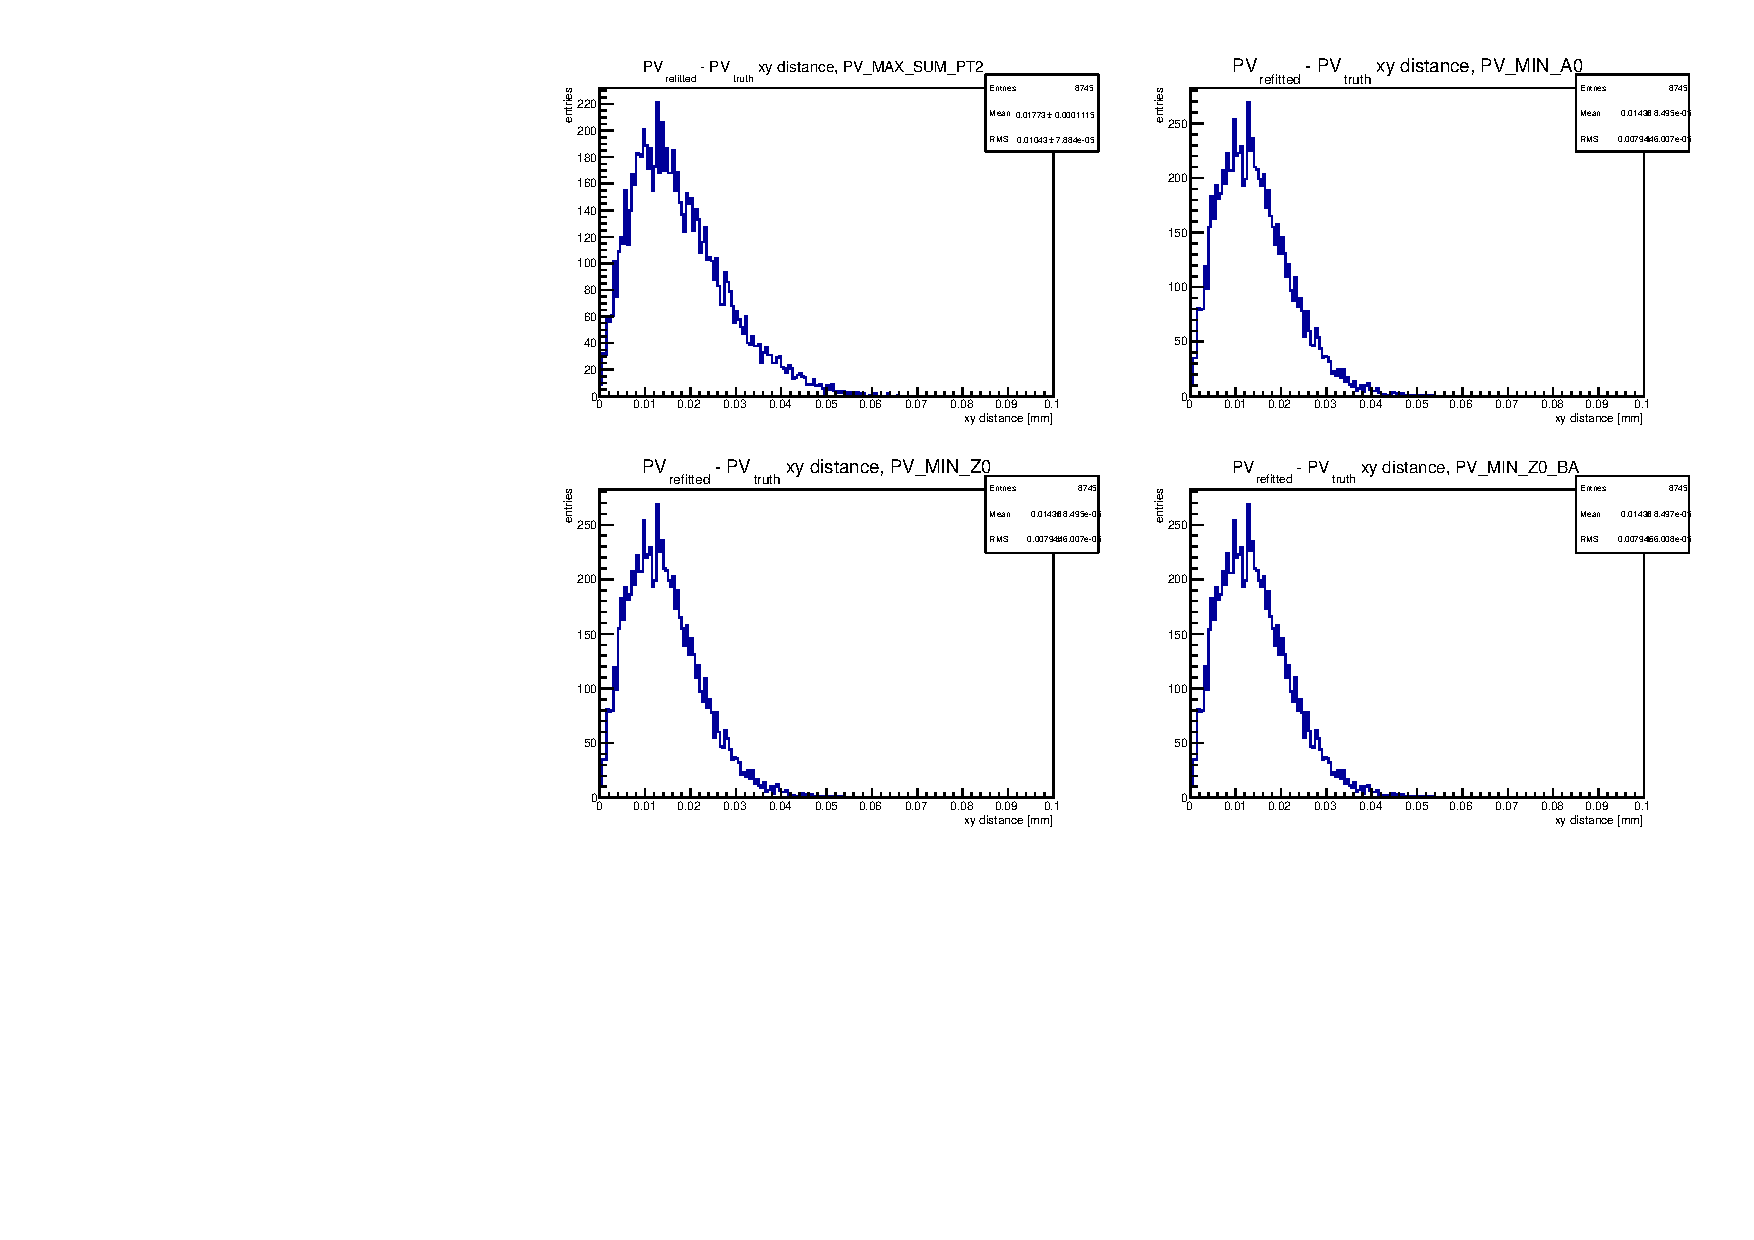
\includegraphics[width=15cm]{figures/InternalNote_Preselection/ref_xy_distance.pdf}
  \caption{xy distance between selected PV and truth PV for the four approaches.}
  \label{fig:PVSVass_xydist}
\end{figure}

\begin{figure}[h]
  \centering
  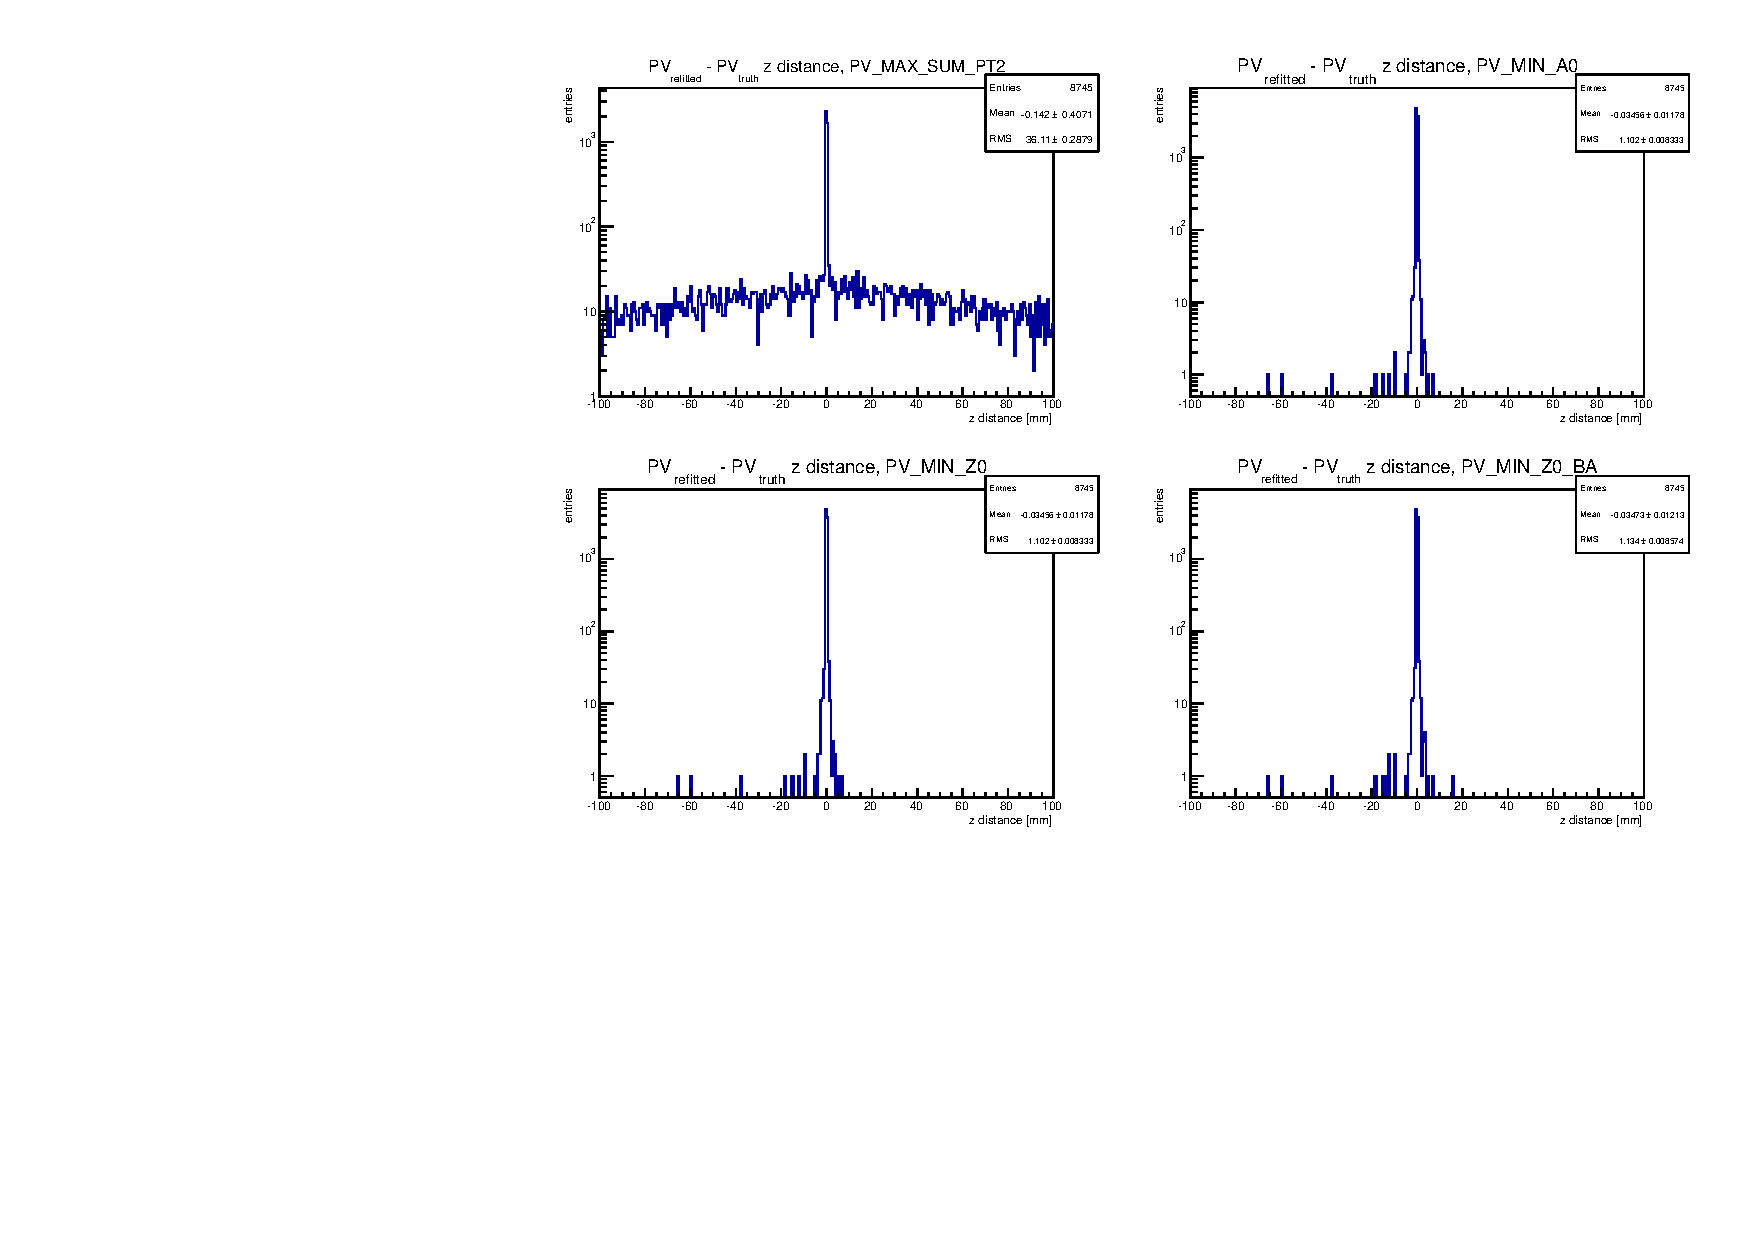
\includegraphics[width=15cm]{figures/InternalNote_Preselection/z_ref_distance_wide.pdf}
  \caption{z distance between selected PV and truth PV for the four approaches.}
  \label{fig:PVSVass_zdist}
\end{figure}

\begin{figure}[h]
  \centering
  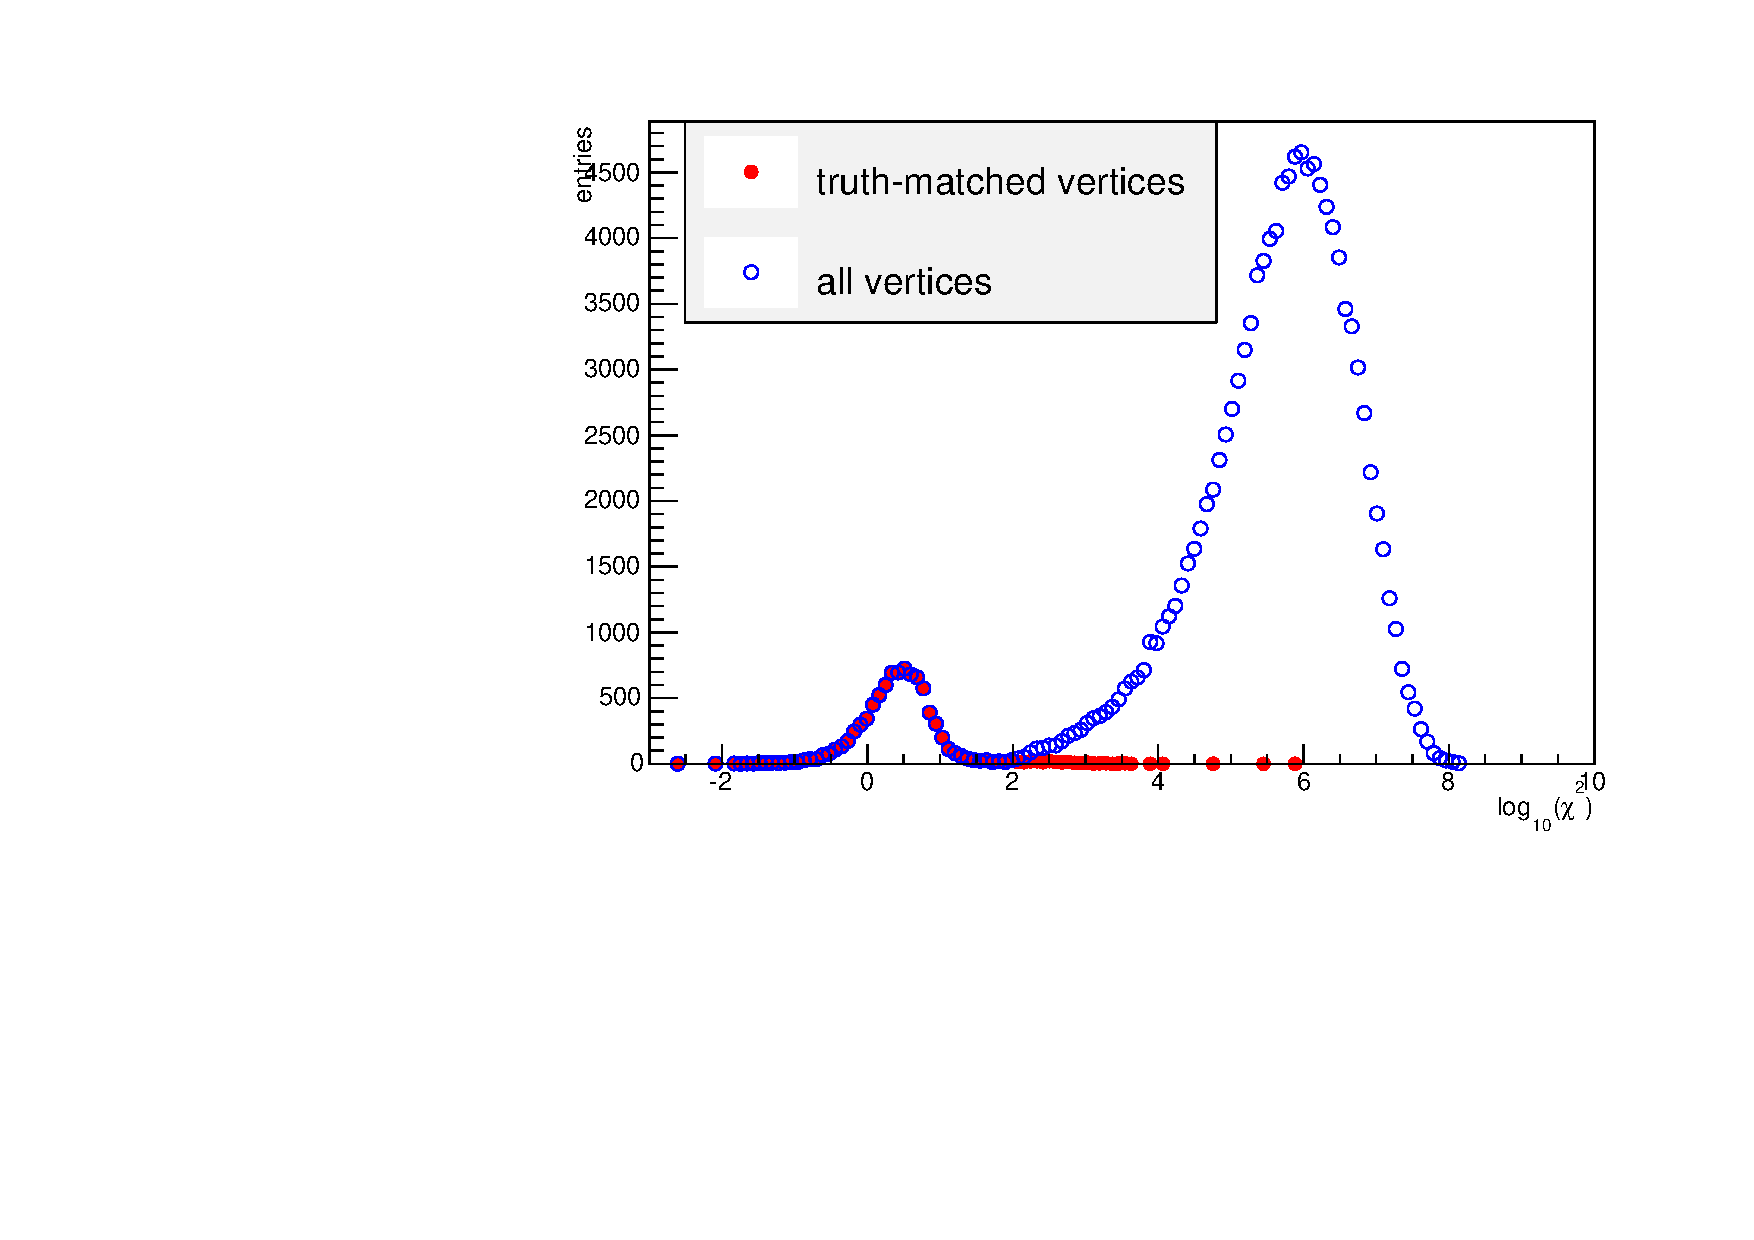
\includegraphics[width=15cm]{figures/InternalNote_Preselection/chi2DistAndMatched.pdf}
  \caption{$\chi^2$ of all the PVs (blue points) and the distribution of the $\chi^2$ of the “truth-matched” PVs.}
  \label{fig:Chi2DistAndMatched}
\end{figure}

\begin{figure}[h]
  \centering
  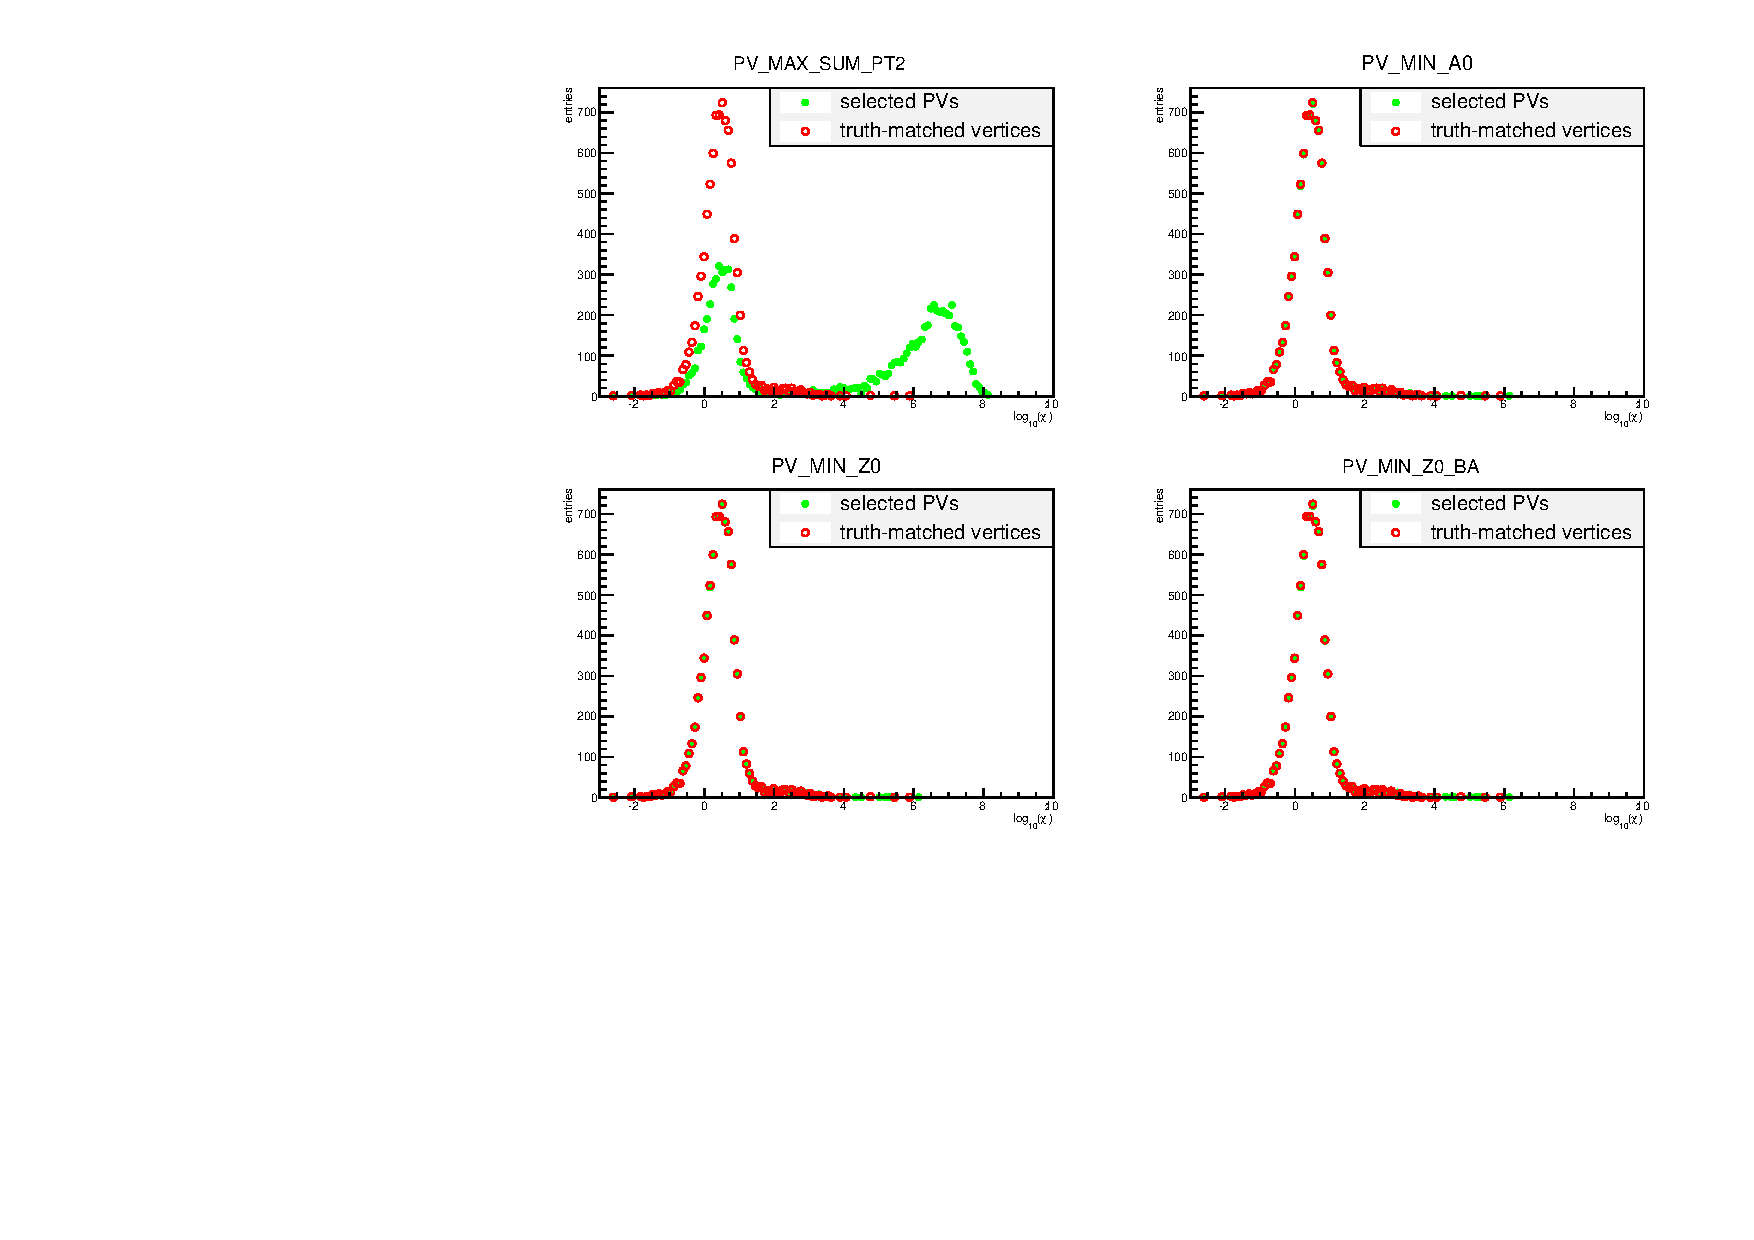
\includegraphics[width=15cm]{figures/InternalNote_Preselection/selectedChi2AndMatched.pdf}
  \caption{$\chi^2$ distribution of the chosen PVs using the 4 approaches (green distributions) superimposed to the truth-matched distribution (red).}
  \label{fig:selectedChi2AndMatched}
\end{figure}

\begin{figure}[h]
  \centering
  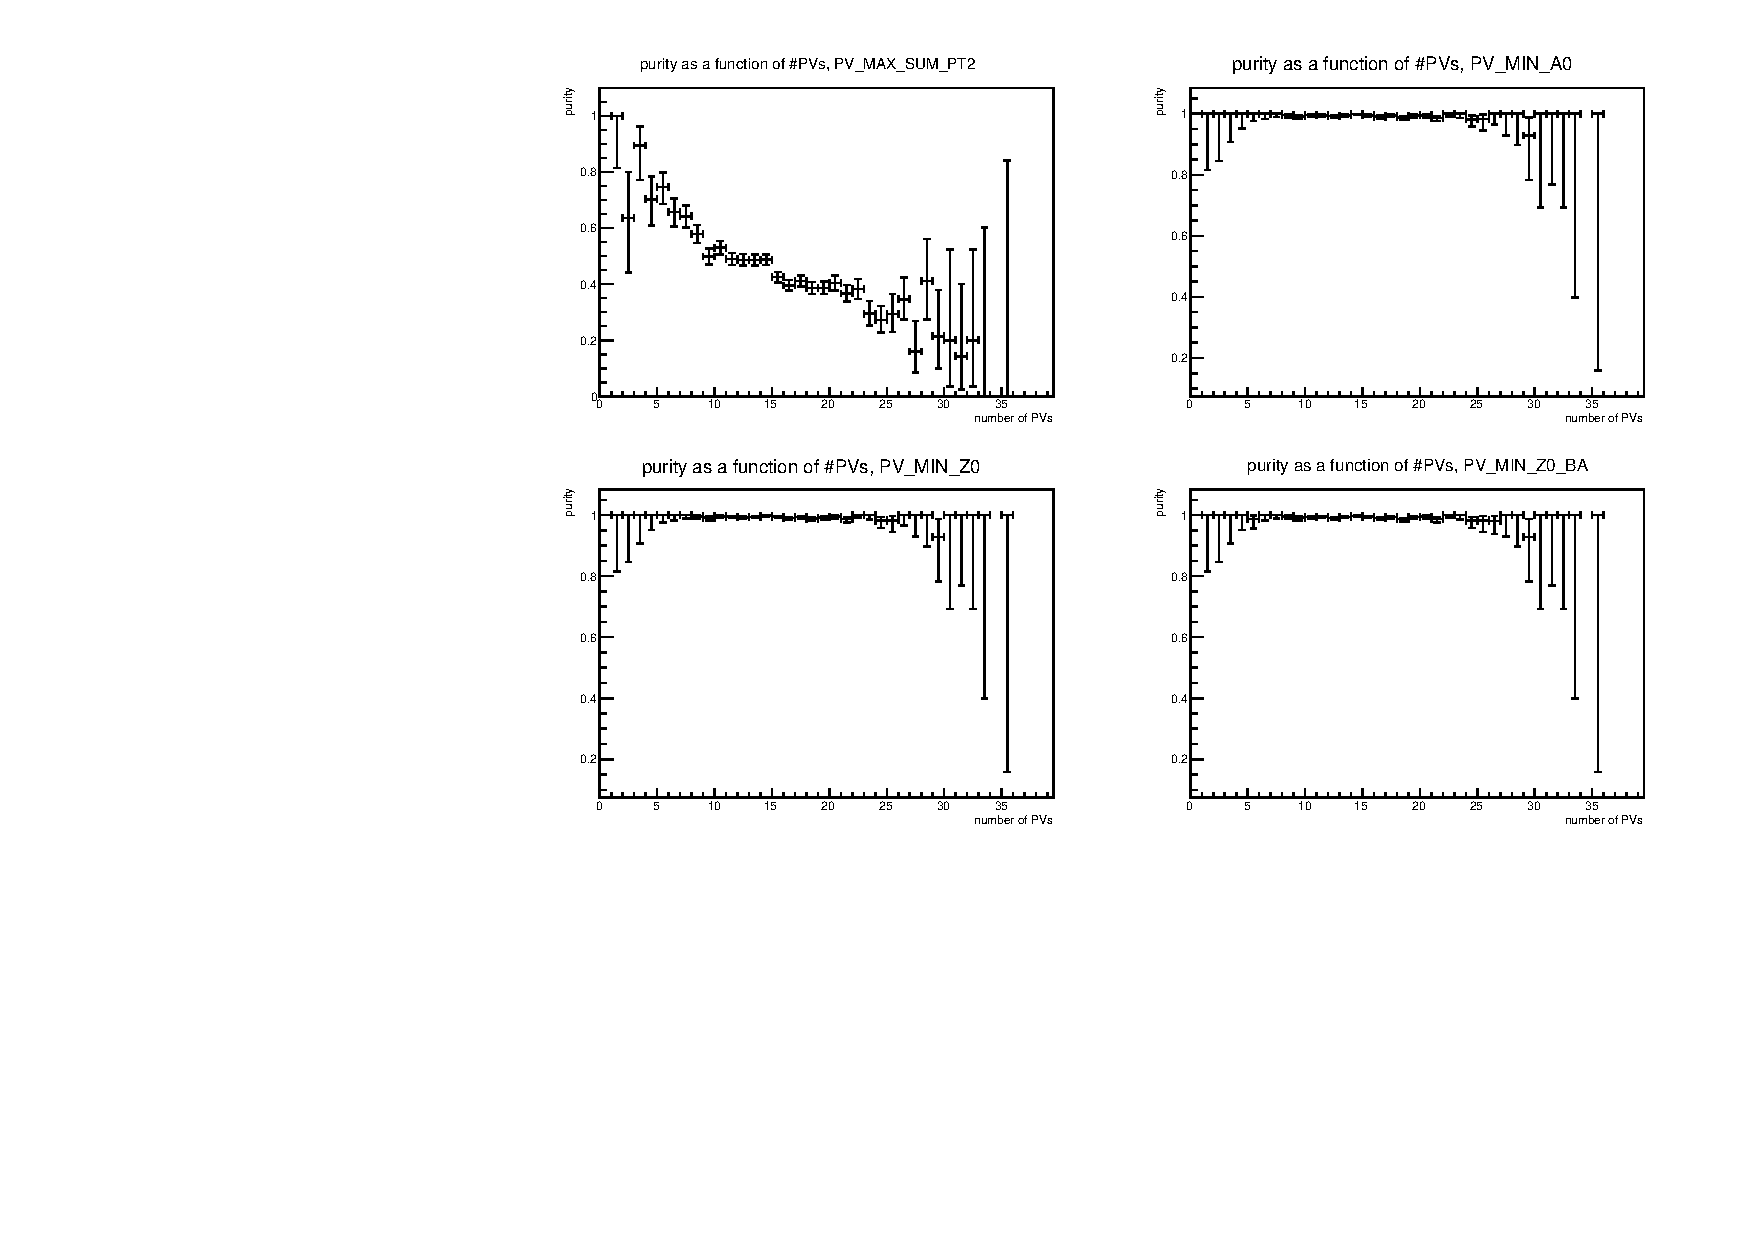
\includegraphics[width=15cm]{figures/InternalNote_Preselection/purityFuncNPV.pdf}
  \caption{purity as a function of number of reconstructed PVs for the four approaches.}
  \label{fig:purityFuncNPV}
\end{figure}



\clearpage
